\documentclass[11pt]{beamer}
\usepackage[utf8]{inputenc}
\usepackage[T1]{fontenc}
\usepackage[magyar]{babel}
%\usetheme{default}
\usetheme{Madrid}

\usepackage[export]{adjustbox}
\usepackage{graphicx}
\graphicspath{{./img/}}


\newcommand{\sumn}[1]{\sum\limits_{{#1}=1}^{n}}


\author{Bálint Márton}
\title[Diplomamunka]{Biztonsági nyomatok eredetiségének ellenőrzése mesterséges neurális hálózatokkal}
%\subtitle{}
%\logo{
\includegraphics[width=10pt]{elte-cimer.jpg}}
\institute[ELTE]{Eötvös Loránd Tudományegyetem}
\date{2018. január 29.}
%\subject{}
%\setbeamercovered{transparent}
%\setbeamertemplate{navigation symbols}{}


\begin{document}
	
\begin{frame}[plain]
	\maketitle
\end{frame}

\begin{frame}
	\frametitle{Motiváció}
	
	\begin{itemize}
	\item 
		Hamisítás
		
		A pénzeket, dokumentumokat hamisítják, ezek eredetiségét ellenőrizni kell.
		
	\item 
		Módszerek a hamisítás ellen:
	
		\begin{enumerate}
			\item
			Az utca embere által ellenőrizhető védelem
			
			(Vízjel, hologramcsík, dombornyomás, stb.)
			
			\item
			Speciális eszközzel, képzett emberek által ellenőrizhető védelem
			
			(Pl. UV tinta)
		\end{enumerate}
		
	\item 
		Köztes megoldás:
		
		Az ellenőrizendő nyomatot egy okostelefonnal lefényképezzük, majd azon egy applikáció kiértékeli az eredményt. 
		
			\begin{enumerate}
			\item
			Mindenki számára elérhető
			
			\item
			Szakértelmet visz az ellenőrzésbe
			
		\end{enumerate}
		
		Ilyen alkalmazást fejlesztett például a Jura Trade Kft.\footnote{http://jura.hu}. 
		
		
	\end{itemize}

\end{frame}

\begin{frame}
	\frametitle{Tanító adatok}
	
	Bementi képek: \textit{(Kb. 1000 darab)}
	\begin{columns}[t]
		
		\begin{column}{.5\textwidth}
			
\includegraphics[width=0.8\textwidth, center]{img/eredeti-pelda.png}
			\centering
			Eredeti
		\end{column}
		\begin{column}{.5\textwidth}
			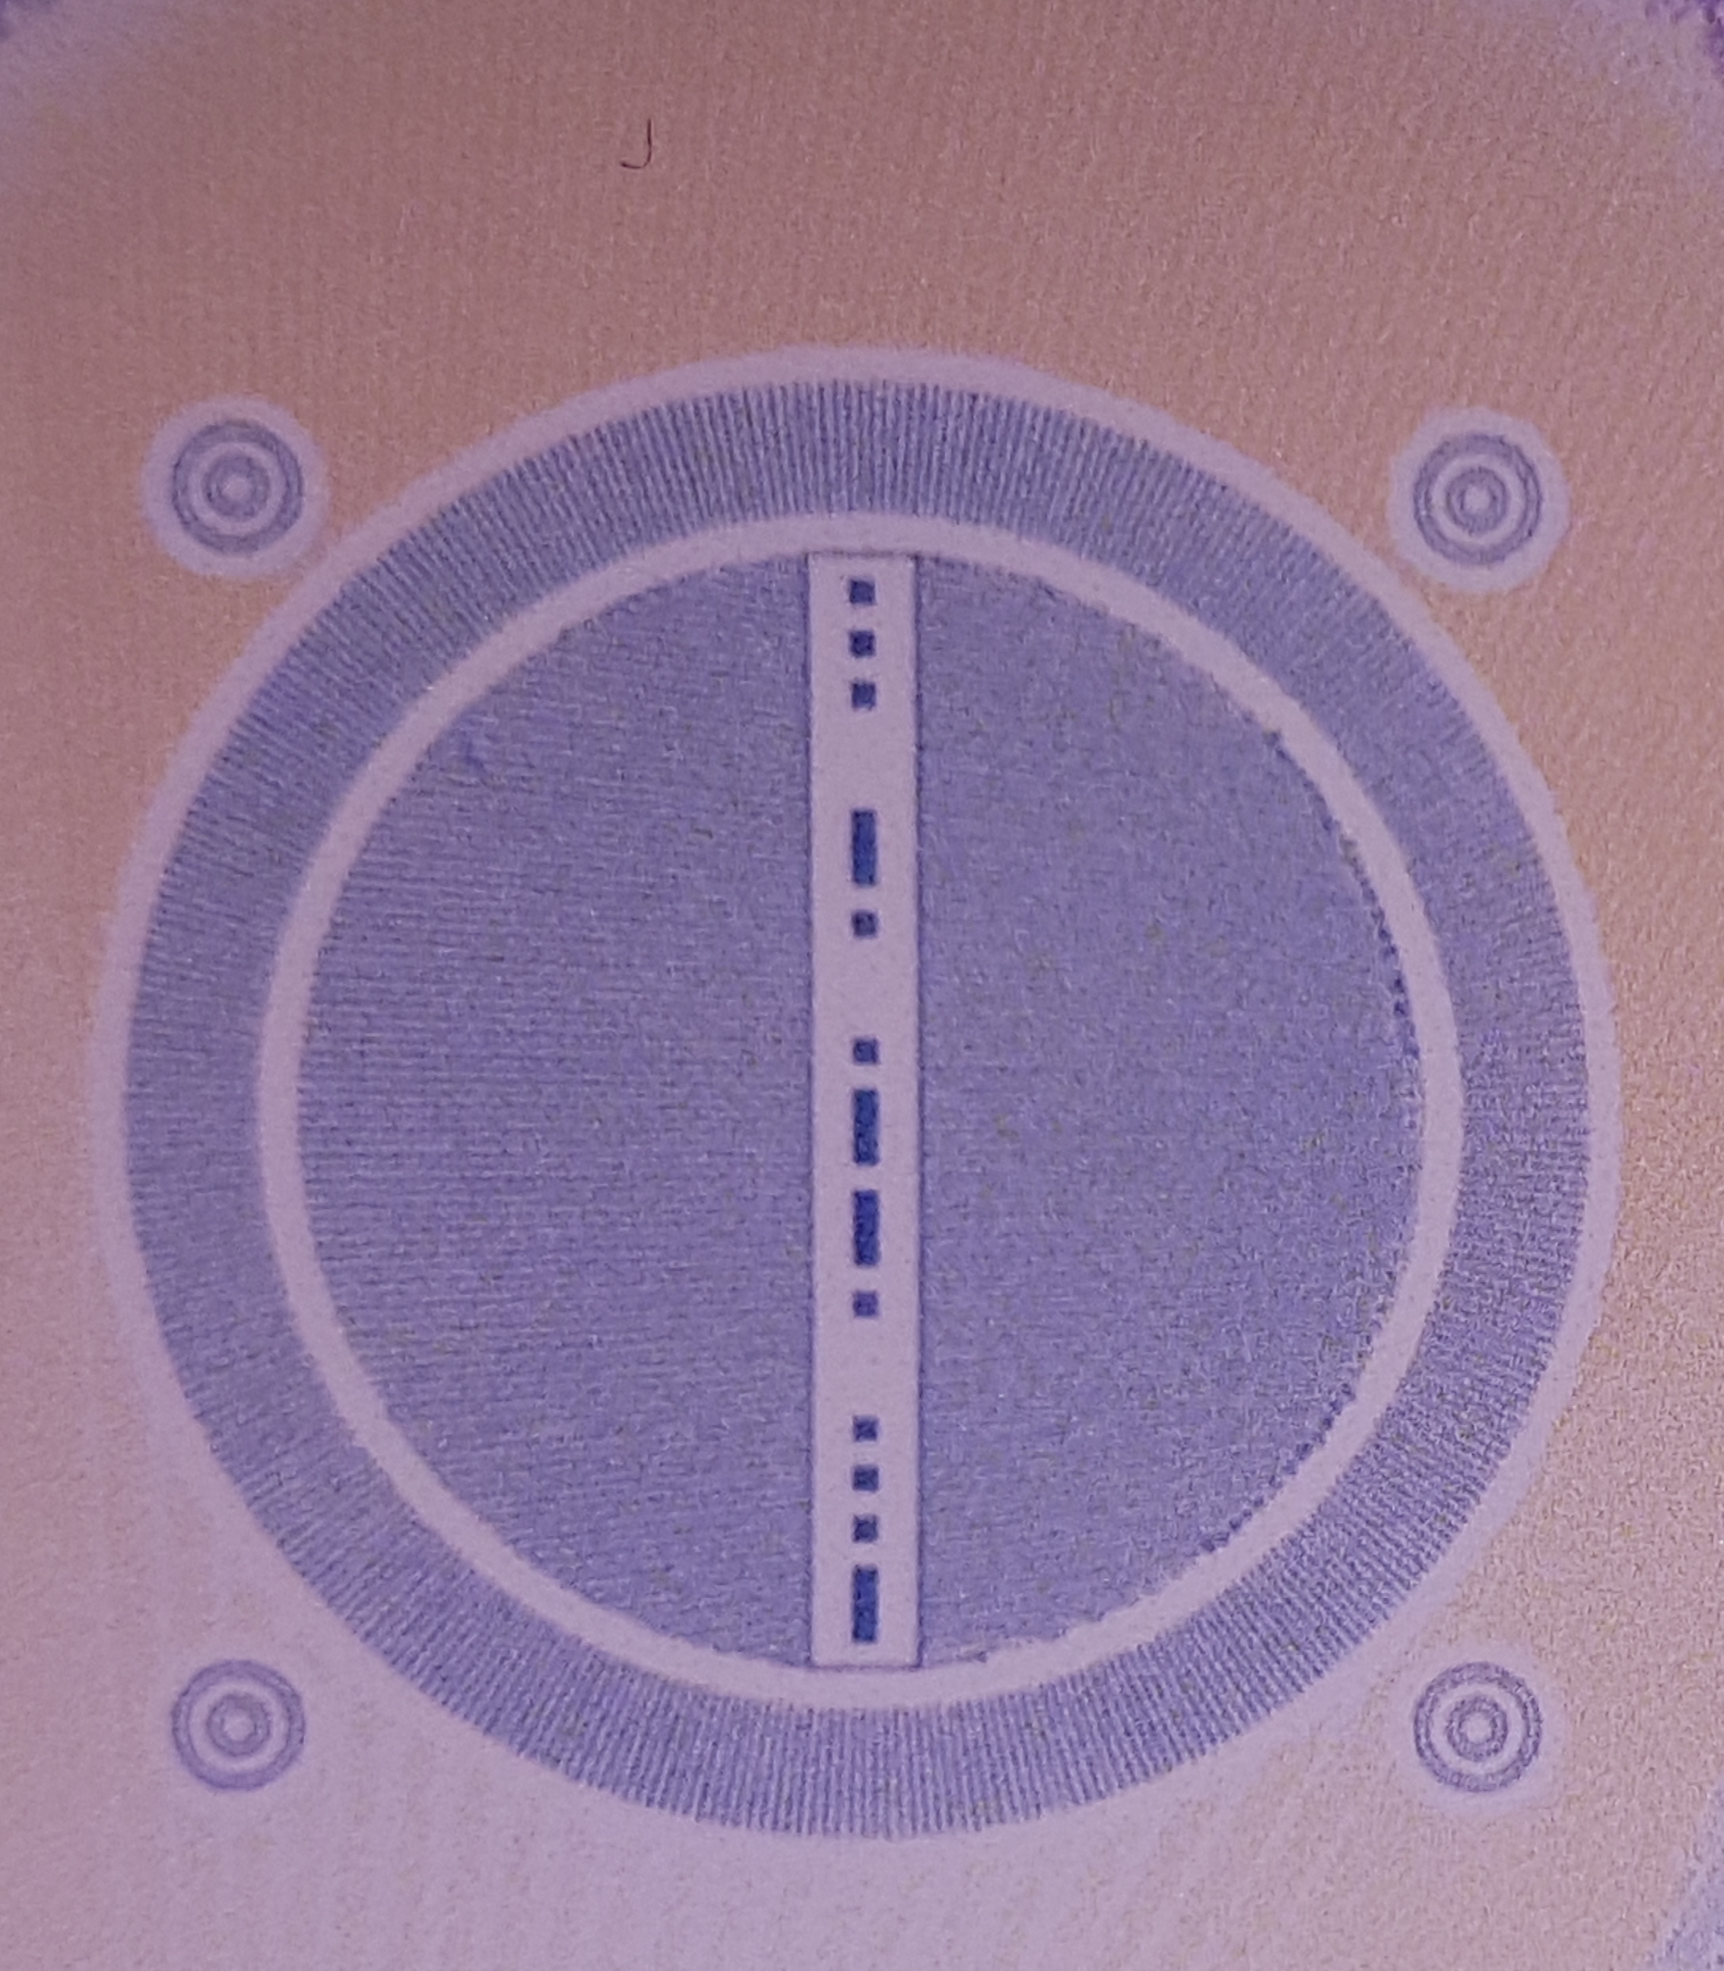
\includegraphics[width=0.8\textwidth, center]{img/copy-pelda.png}
			
			\centering
			Fénymásolat
			
		\end{column}				
	\end{columns}
	
	
	
	%	
	%	\begin{figure}[h]
	%		
	%		
	%		
	%		\begin{minipage}[c]{0.5\linewidth}
	%			\centering
	%			
\includegraphics[width=\textwidth]{img/eredeti-pelda.png}
	%			\caption{Egy eredeti nyomat.}
	%			\label{fig:eredeti.pelda}
	%			
	%		\end{minipage}\hfill
	%		\begin{minipage}[c]{0.5\linewidth}
	%			\centering
	%			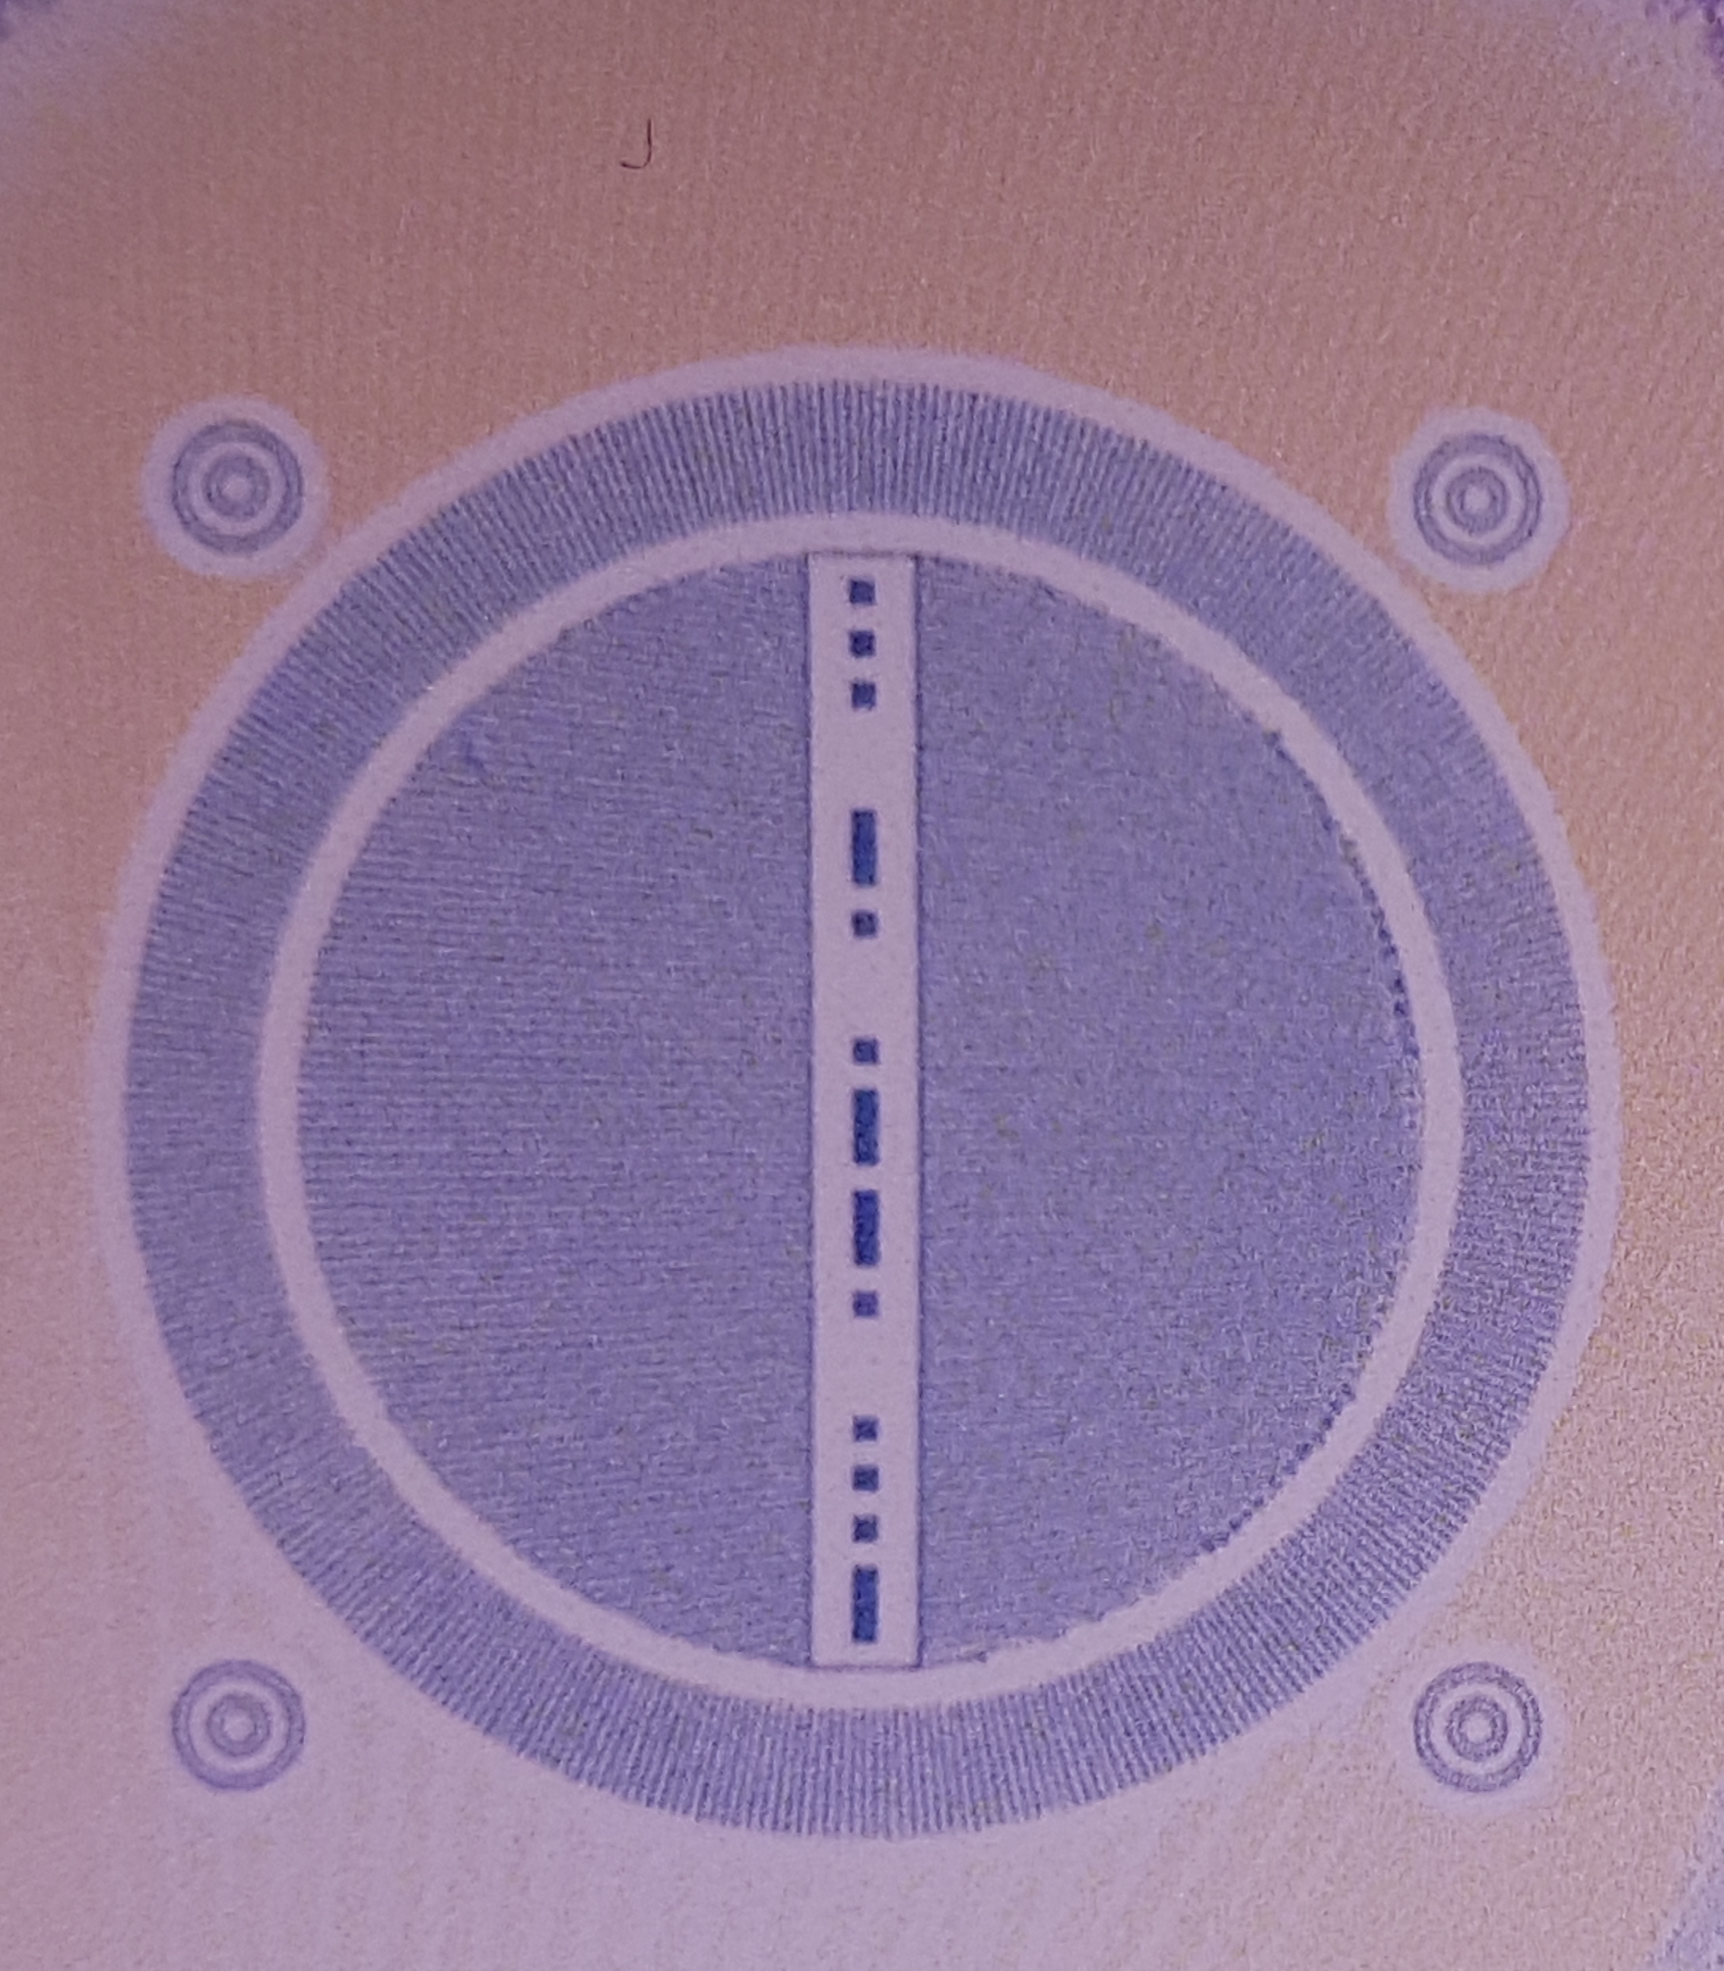
\includegraphics[width=\textwidth]{img/copy-pelda.png}
	%			\caption{Egy színes fénymásolat.}
	%			\label{fig:copy.pelda}
	%			
	%		\end{minipage}
	%		
	%	\end{figure}

\end{frame}

\begin{frame}
	\frametitle{Ötlet}
	
	
	\begin{itemize}
		\item 
		Az említett alkalmazás méréseket végez a képen, ezekből 10-20 mérőszámot állít elő, majd ezek alapján ad eredményt, hogy a kép eredeti, hamis, vagy nem tudja eldönteni.
		
		\item 
		A dolgozat célja az volt, hogy ezt az alkalmazást továbbfejlesszük különböző gépi tanulási módszerekkel.
		
		
	\end{itemize}
\end{frame}




\begin{frame}
	\frametitle{Gépi tanulás}
	\framesubtitle{Használt módszerek}
	
	
	\begin{block}{A kanonikus tanulási feladat}
			\[ 
		\min\limits_{\underline{\theta}} L(\underline{\theta}, \underline{x}_1, \dots, \underline{x}_n, \underline{y}_1, \dots, \underline{y}_n) = \frac{1}{n}  \sumn i l\big(f(\underline{\theta}, \underline{x}_i), \underline{y}_i\big) + R(\underline{\theta})
		, \]
	\textit{$ \theta $: tanulandó paraméterek, $ l $: költségfüggvény, $ f $: modell, $ R $: regularizáció}
	\end{block}


	
	Általunk használt modellek:
	\begin{itemize}
	\item 
		Felügyelt tanulás
		
		\begin{enumerate}
		\item 
			SVM	
		\item 
			Mély konvolúciós háló
		
		\end{enumerate}
		
	\item 
		Felügyelet nélküli tanulás
		
		\begin{enumerate}
		\setcounter{enumi}{2}
		\item 
			Konvolúciós autoencoder
		\end{enumerate}		
		
	\end{itemize}
\end{frame}




\begin{frame}
	\frametitle{Support Vector Machine (SVM) - Támasztóvektor Gép}
	\framesubtitle{Rövid áttekintés}
		
	Feladat: 
	
	Adott $ \underline{x}_i $ jellemzők, $ \underline{y}_i $ bináris osztályok, 
	határozzunk meg egy $ (\underline{x}, b) $ hipersíkot úgy, hogy: 
	
	\[
	\begin{cases}
	\underline{x}_i^T \underline{w} - b \geq +1, & \text{ ha }  y_i=1, \\
	\underline{x}_i^T \underline{w} - b \leq -1, & \text{ ha }  y_i=-1.
	\end{cases}
	\]	
	
	Ennek megoldásához a következő kifejezést kell minimalizálnunk:
	
	\[
%	L(\underline{\theta}, \underline{x}_1, \dots, \underline{x}_n, y_1, \dots, y_n)  = 
%	\frac{1}{n} 
	\min_{\underline{w},b}
	\sum\limits_{i=1}^{n} 
	%\max\big(0, 1 - y_i(\underline{w} \cdot \underline{x}_i - b)\big) + \lambda \norm{\underline{w}}_2^2.
	\max\big(0, 1 - y_i(\underline{w}^T \underline{x}_i - b)\big) + \lambda \lvert\underline{w}\rvert_2^2.
	\]
	
	
	
\end{frame}

\begin{frame}
	\frametitle{Support Vector Machine (SVM) - Támasztóvektor Gép}
	\framesubtitle{Rövid áttekintés}
	
	Belátható, hogy ez a következő kvadratikus programozási feladatra vezethető vissza:
	\begin{multline*}
	\max\limits_{\underline{c}} \sum\limits_{i=1}^{n}c_i -  
	\frac{1}{2}\sumn{i}\sumn{j} y_i c_i (\underline{x}_i^T \underline{x}_j) y_i c_j \\
	\text{ s.t. } \quad 
	\sumn{i} c_i y_i = 0, \quad
	0 \leq c_i \leq \frac{1}{2n\lambda}, \quad 
	i=1,\dots,n.
	\end{multline*}
	
	Ekkor a keresett paraméterek:
	\[
	\underline{w} = \sumn{i} c_i y_i \underline{x}_i.
	\]
	
%	Keressünk egy margón lévő $ (\underline{x}_i, y_i) $ párt:
%	\[
%	b = \underline{w}^T \underline{x}_i  - y_i.
%	\]
	
	\textit{Megjegyzés: Ha nem tökéletesen szeparálható a két adathalmaz, akkor $ b $ megfelelő választásával lehet részrehajlást (bias) állítani.}
\end{frame}




\begin{frame}
	\frametitle{SVM - Kernel trükk}
	\framesubtitle{Rövid áttekintés}
	\textbf{Nemlineáris osztályozás:}
	
	Megnöveljük a bemenetünk dimenzióját úgy, hogy új értékeket számolunk ki az előzőek alapján. Ehhez definiáljuk a következő függvényt:
	\[
	\varphi\colon \mathbb{R}^p \rightarrow \mathbb{R}^q, \quad q \gg p.
	\]
	
	Ezután $ x_i $ minta helyett $ \varphi(x_i) $ bemenettel számolunk.
	
	\textbf{Kernel trükk: }
	
	A feladatban szereplő $ k(\underline{x}_i, \underline{x}_j) := \varphi(\underline{x}_i)^T \varphi(\underline{x}_j) $ skaláris szorzatot bizonyos esetekben akkor is ki tudjuk hatékonyan számolni, ha $ \varphi(x_i) $ dimenziója nagy, vagy esetleg végtelen. (Ekkor $ k $-t nevezzük \textit{kernelnek}.)
%	\[
%	k(\underline{x}_i, \underline{x}_j) = \varphi(\underline{x}_i)^T \varphi(\underline{x}_j).
%	\]
	


\end{frame}

%\begin{frame}
%	\frametitle{Support Vector Machine (SVM) - Támasztóvektor Gép}
%	
%	%A cél az volt, hogy az eredeti alkalmazás által számolt jellemzőkből hozzunk döntést.
%	
%
%	\begin{enumerate}
%	\item 
%		
%	\end{enumerate}		
%
%
%\end{frame}


\begin{frame}
	\frametitle{SVM - Alkalmazás}
	
	Mi az SVM-et arra használjuk, hogy az említett alkalmazás által számolt jellemzőkből gépi tanulás segítségével hozzunk döntést.
	\begin{block}{Megjegyzés}
		Az jellemzőket fekete doboznak tekintjük, nem használjuk fel a mögöttes tartalmukat. A cél, hogy az algoritmus magától találjon összefüggéseket.
	\end{block}

	Az alkalmazás eredményeit egy \texttt{.csv} fájlból töltjük be \texttt{python} segítségével. Az osztályozást az \texttt{sklearn} csomaggal végezzük.

\end{frame}


\begin{frame}
	\frametitle{SVM - Eredmények}
	\framesubtitle{Fals pozitív(FP) és fals negatív(FN) hibarátákkal}
	
	\begin{figure}[h!]
		\centering
		\begin{tabular}{ l c c c c }
			\underline{Módszer} 		& Összes minta 	& Bizonytalan	& FP	& FN \\
			\texttt{bpas-verdict.csv} 	& 959 			& 0.21			& 0.10215 	& 0.00905 	\\
			\texttt{bpas-merged.csv}\footnote{Egymás után készült két kép közül a jobb eredmény} 	& 496			& 0.10			& 0.14545 	& 0.00259   \\
			
			\hline
			(1) verdict+SVM					& 894			& 0				& 0.00297	& 0.00566	\\
			(2) merged+SVM					& 453			& 0				& 0.01493	& 0.00771	\\
			(3) verdict+SVM 2 képpel		& 423			& 0				& 0.01420	& 0.01059   \\
			
		\end{tabular}
		
		%	\begin{flushleft}
		%	\textit{*Lásd a \ref{sec:adatok} pontot.}
		%	\end{flushleft}
		\caption{Az SVM eredményei összehasonlítva az eredeti algoritmusokéval.}
		
	\end{figure}

	Összességében elmondható, hogy az SVM jobban teljesített a manuálisan gyártott algoritmusoknál.
	
\end{frame}


\begin{frame}
	\frametitle{Mély konvolúciós hálók}
	\framesubtitle{Rövid áttekintés}
	
	Egy mély háló egy paraméterezett, többszörösen összetett függvény, amely elvárás szerint a bemenetet az elvárt kimenetre képzi. A belső paramétereket gradiens módszer segítségével optimalizáljuk.
	
	Jellemző rétegek:
%	\begin{enumerate}
%	\item
%		Sűrű réteg
%	\item 
%		Konvolúciós réteg
%	\item 
%		Aktivációs rétegek
%		\begin{itemize}
%		\item 
%			ReLU
%		\item
%			Softmax
%		\end{itemize}
%	\item 
%		Alul-, felülmintavételező réteg
%	\item 
%		Költségfüggvény\footnote{Nem igazi réteg}
%		\begin{itemize}
%		\item 
%			Keresztentrópia
%		\end{itemize}
%	\end{enumerate}

	\begin{columns}
		
		\begin{column}{.5\textwidth}
				\begin{enumerate}
				\item
				Sűrű réteg
				\item 
				Konvolúciós réteg
				\item 
				Aktivációs rétegek
				\begin{itemize}
					\item 
					ReLU
					\item
					Softmax
				\end{itemize}
				\item 
				Alul-, felülmintavételező réteg
				\item 
				Költségfüggvény\footnotemark 
				\begin{itemize}
					\item 
					Keresztentrópia
				\end{itemize}
			\end{enumerate}
		\end{column}
		\begin{column}{.5\textwidth}
			
			
			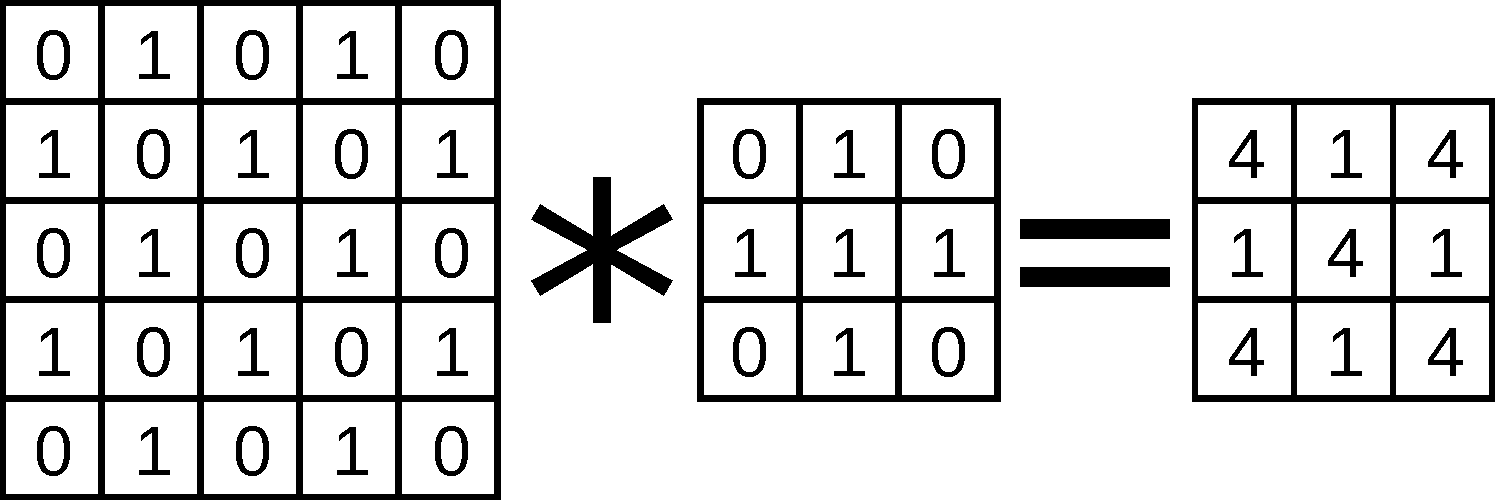
\includegraphics[width=0.8\textwidth]{konv-pelda.pdf}
			
			\centering
			Konvolúció
			
		\end{column}				
	\end{columns}
	\footnotetext{Nem igazi réteg}
	

\end{frame}


\begin{frame}
	\frametitle{Mély konvolúciós hálók}
	\framesubtitle{Alkalmazás}
	
	A bemeneti képek alapján tanítunk egy konvolúciós hálót. A megvalósításhoz a \texttt{python} \texttt{Keras} csomagját használtuk.	
	
	A háló modellje:
	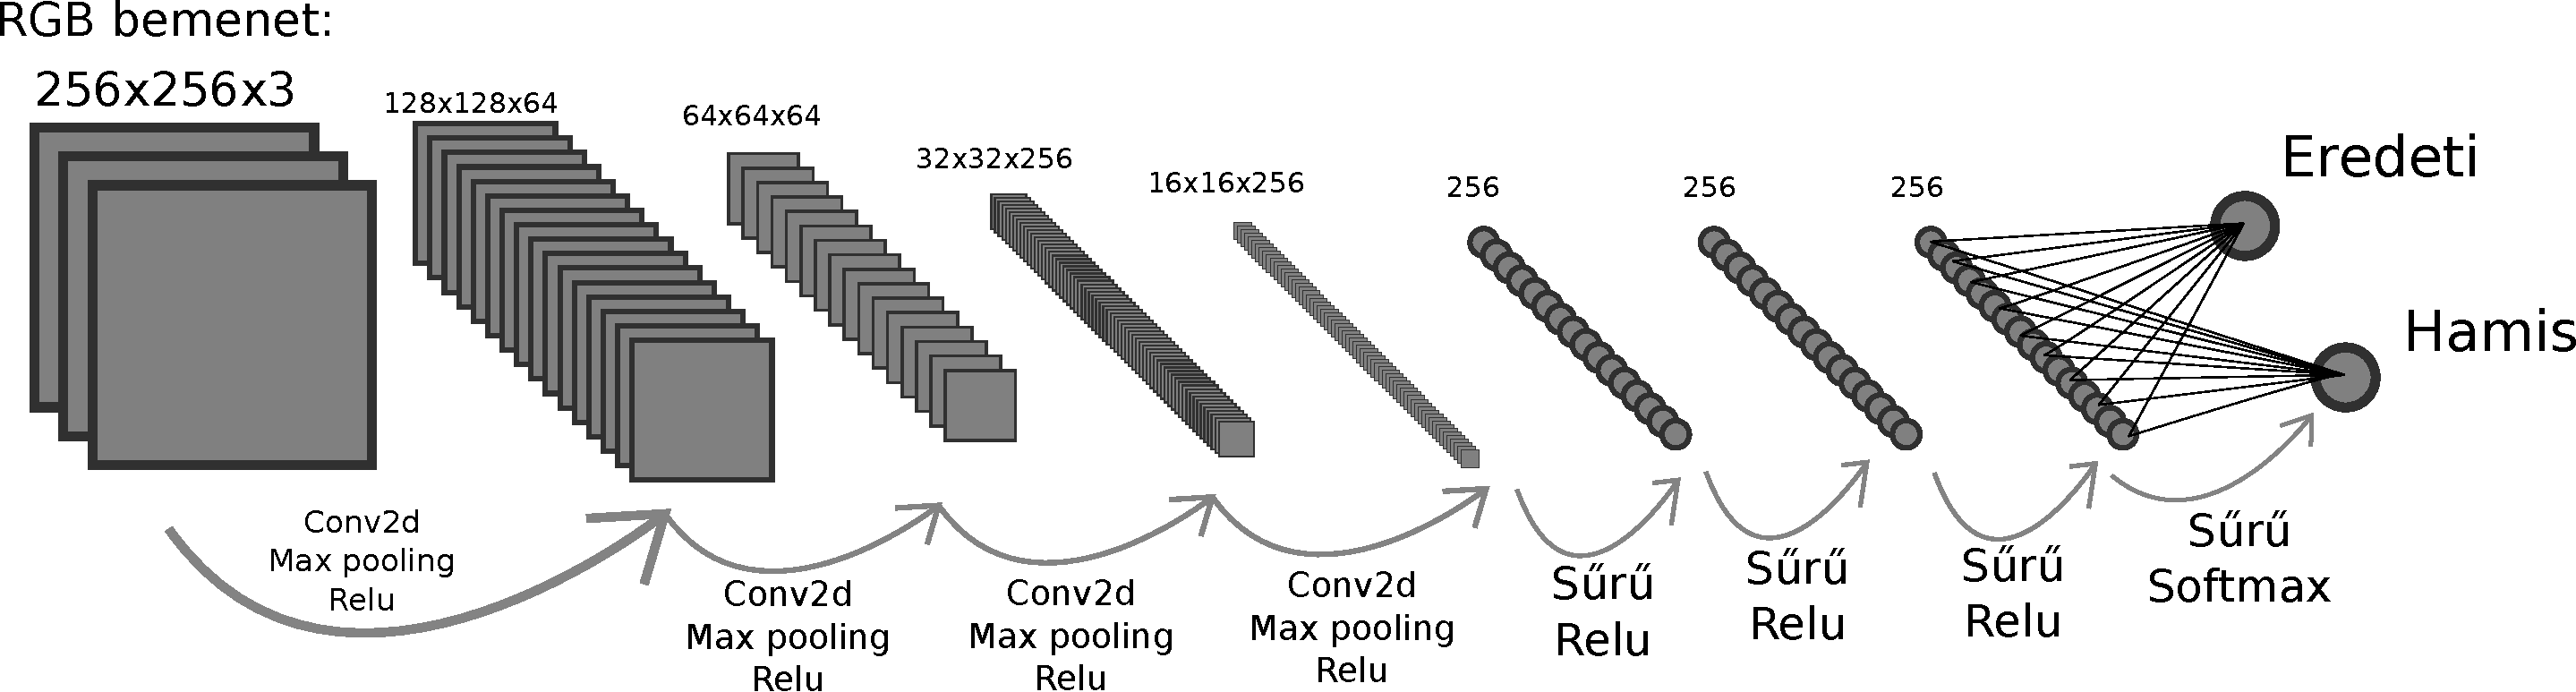
\includegraphics[width=0.8\textwidth, center]{predictor-network-modell.pdf}
	
	
	

%	\begin{columns}
%		\begin{column}{.5\textwidth}
%			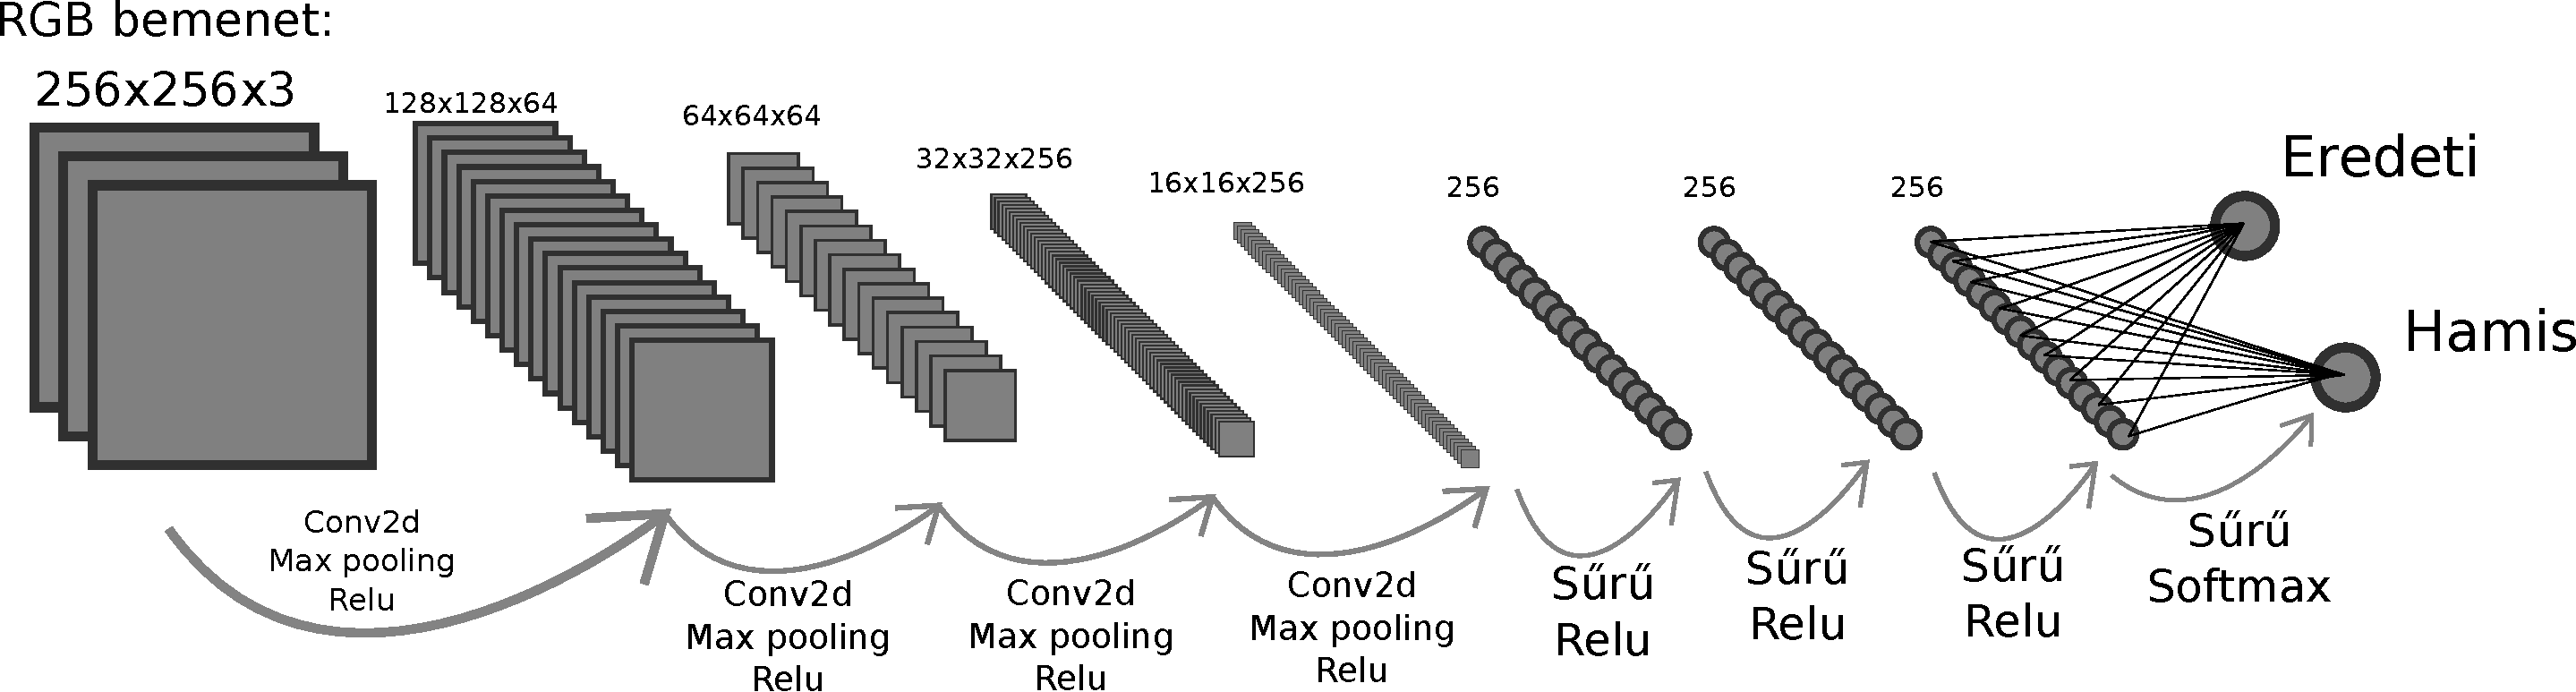
\includegraphics[width=0.8\textwidth, center]{predictor-network-modell.pdf}
%			A bemeneti képek alapján tanítunk egy konvolúciós hálót.
%		\end{column}
%		\begin{column}{.5\textwidth}
%			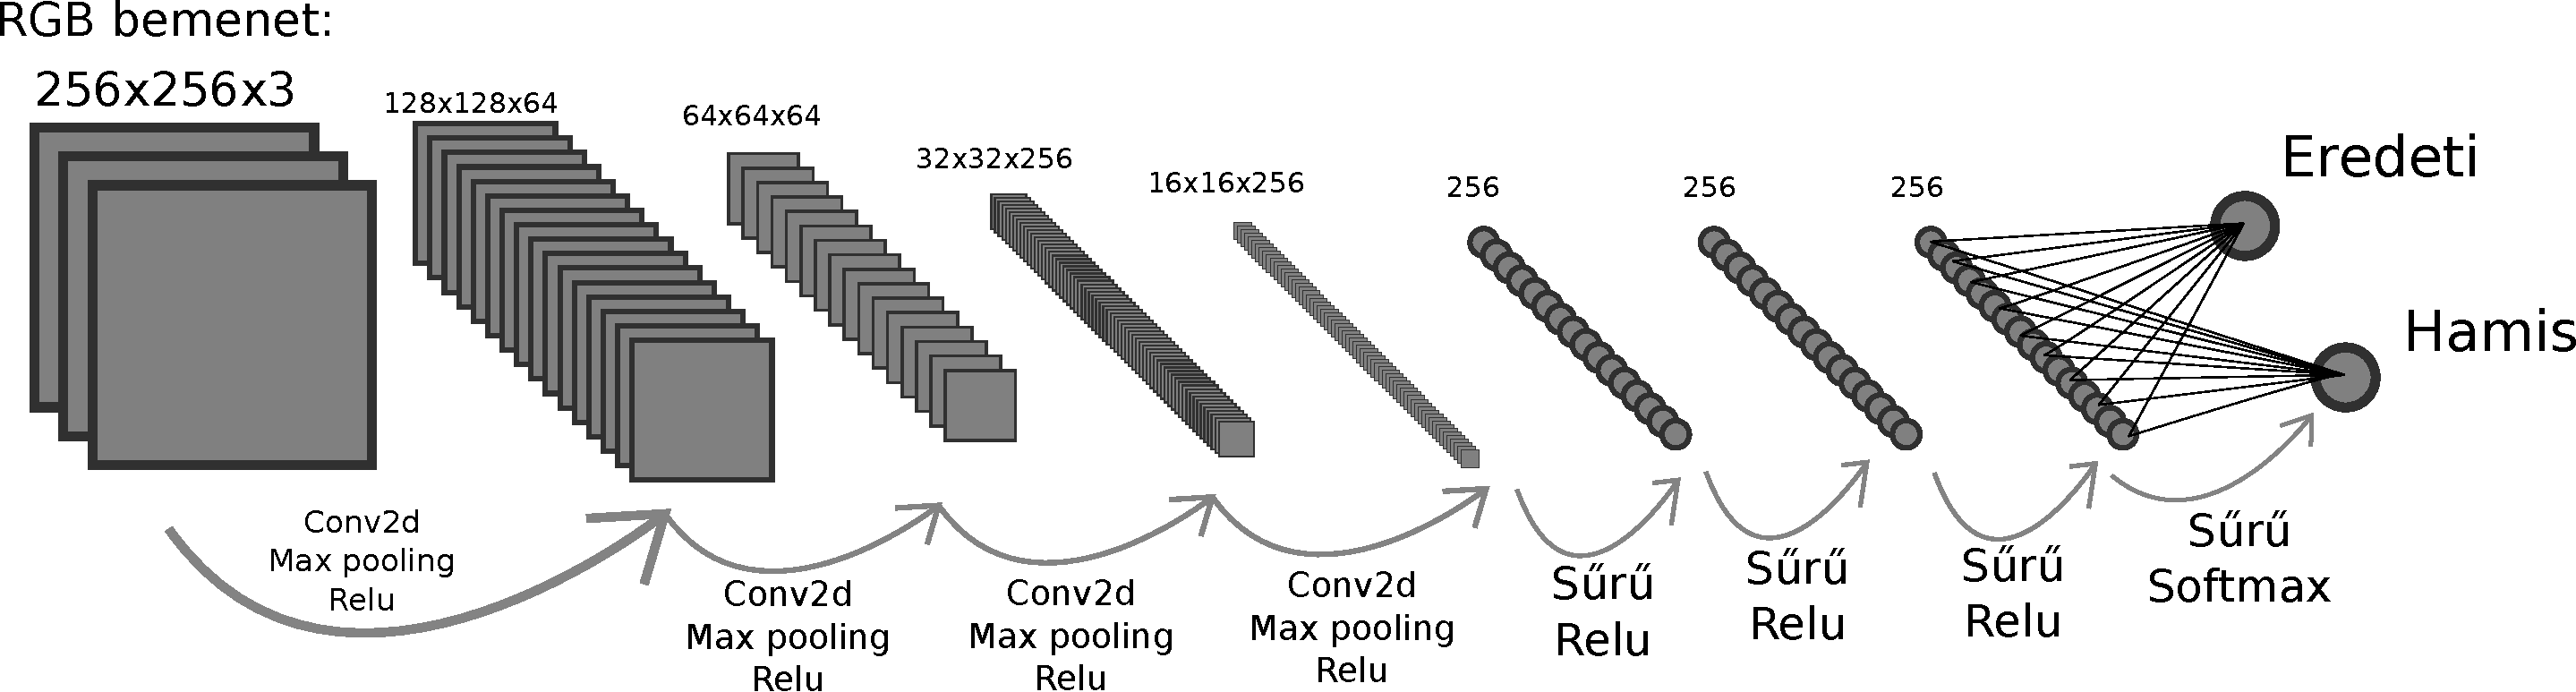
\includegraphics[width=0.8\textwidth, center]{predictor-network-modell.pdf}
%			
%		\end{column}				
%	\end{columns}
	
	

\end{frame}


\begin{frame}
\frametitle{Mély konvolúciós hálók}
\framesubtitle{Kihívások}

\begin{itemize}
	\item 
	Hiperparaméterek beállítása
	\begin{enumerate}
		\item 
		Háló szerkezete
		\item 
		Minibatch-ek mérete
	\end{enumerate}
	
	\item 
	Túltanulás elkerülése
	\begin{enumerate}
		\item 
		Dropout
		\item 
		Adatok mesterséges generálása (augmentation)
	\end{enumerate}
	
\end{itemize}

\end{frame}

\begin{frame}
	\frametitle{Mély konvolúciós hálók}
	\framesubtitle{Kihívások}
	
	\textbf{Lokális szélső értékek}
	
	A gradiens módszer miatt előfordulhat hogy lokális minimumot találunk és a tanítás megáll. Ez előfordult a mi esetünkben is. A probléma alapja az volt, hogy néhány hamisítvány túlságosan hasonlított az eredetiekre, ezért a tanulás rosszul konvergált, és minden képet eredetinek osztályzott. Ezeket a képeket eltávolítva, a módszer stabilan működött. Ezután visszahelyeztük a kritikus eseteket a tanító halmazba, ekkor már jó eredményt adtak.
	
	
\end{frame}

\begin{frame}
	\frametitle{Autoencoder}
	
	Ennek a problémának a felderítésében segített az autoencoder modell:
	
	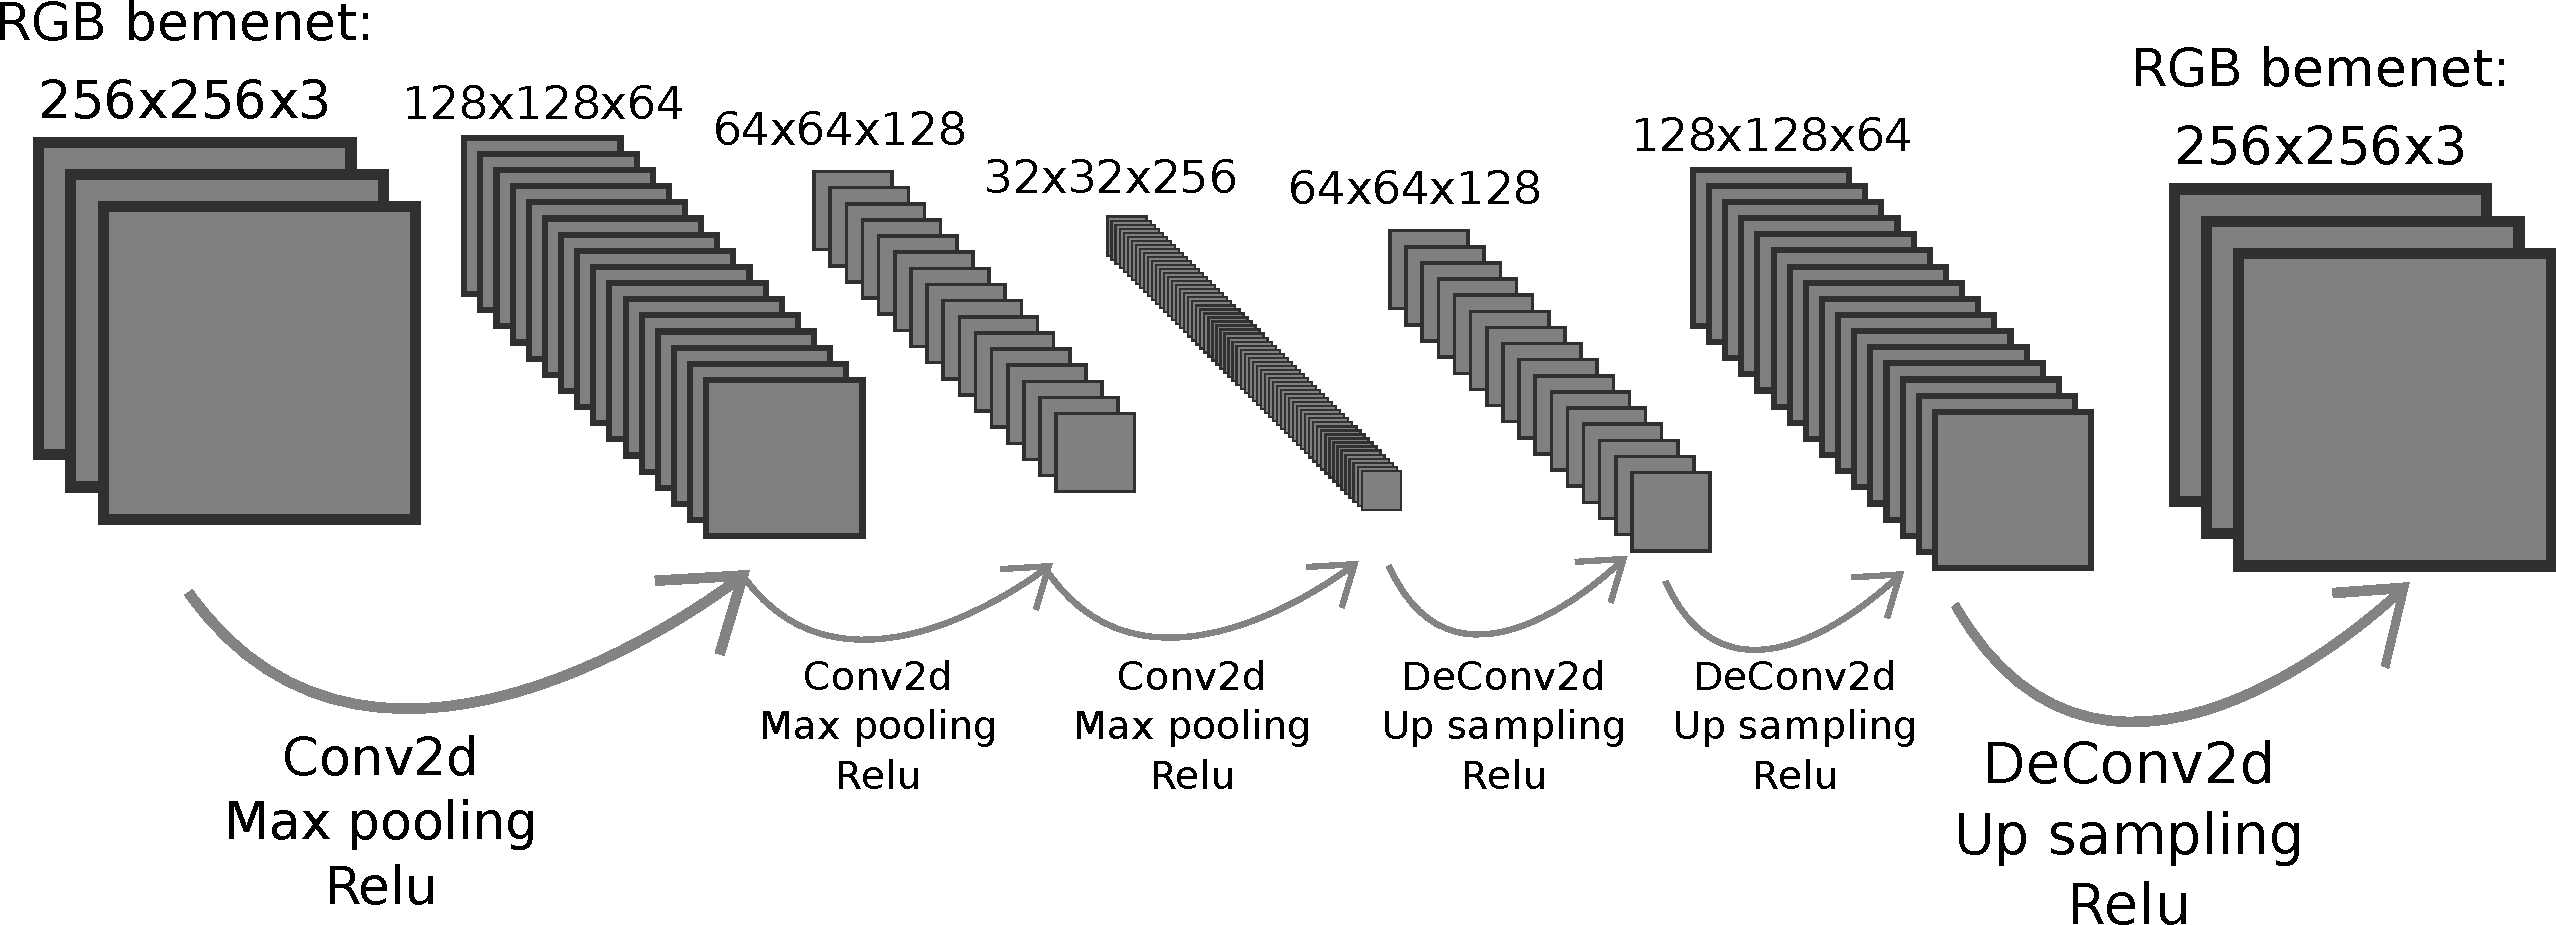
\includegraphics[width=0.8\textwidth]{autoencoder-network-modell.pdf}

	Lényege, hogy a képet konvolúciós rétegek segítségével betömörítjük, majd kitömörítjük, és a rekonstrukciós hibát mérjük, úgy hogy csak az eredeti képeken tanítunk. Azt vártuk, hogy az ismeretlen, azaz hamis képekre a hiba nagyobb lesz.
	
	Ekkor láthatóvá vált, hogy bizonyos hamis képek nagyban hasonlítanak az eredetiekre.
	
	Bár a módszer működik, messze nem olyan hatékony mint az előző, predikciós mély háló.
	
	



\end{frame}


\begin{frame}
	\frametitle{Mély konvolúciós hálók}
	\framesubtitle{Eredmények}
	
	
	
	
	
	\begin{columns} [t]
		\begin{column}{.5\textwidth}
			\centering
			Teszt adathalmaz
			
			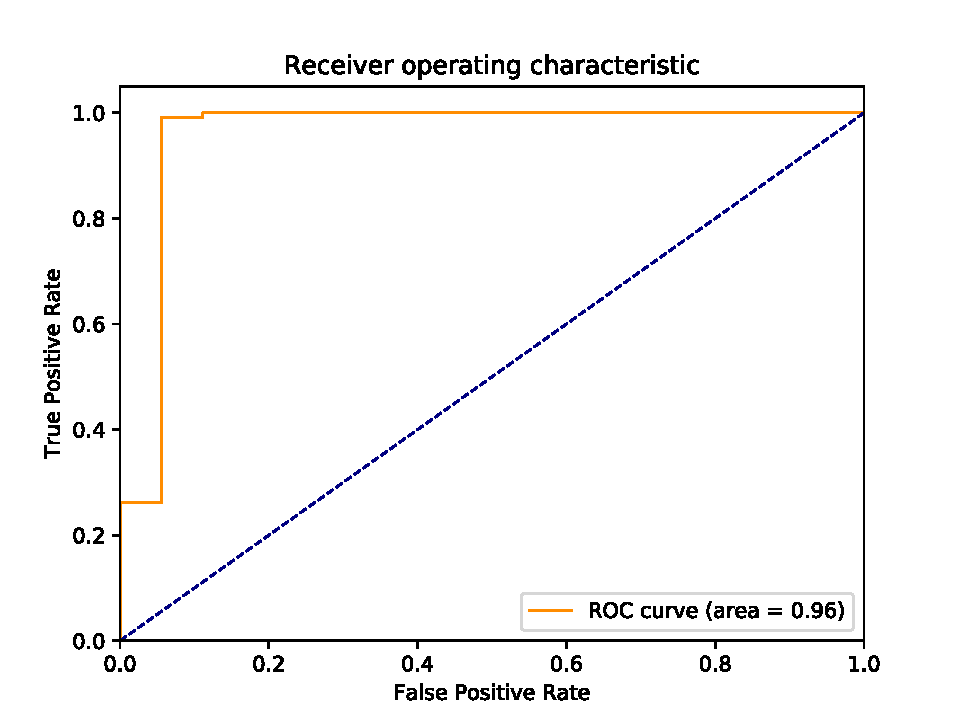
\includegraphics[scale=0.25]{ruc-curve-test-ujratanitva.pdf}
			
			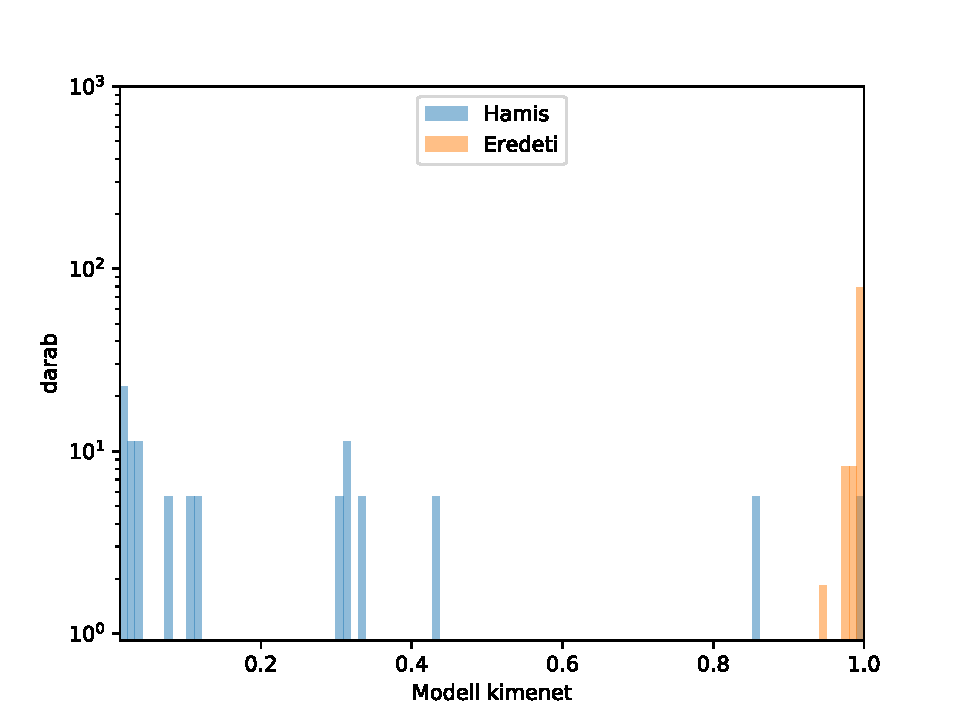
\includegraphics[scale=0.25]{histogram-ujratanitott-log-skala-test.pdf}
			
		\end{column}
		\begin{column}{.5\textwidth}
			\centering
			Teljes adathalmaz
			
			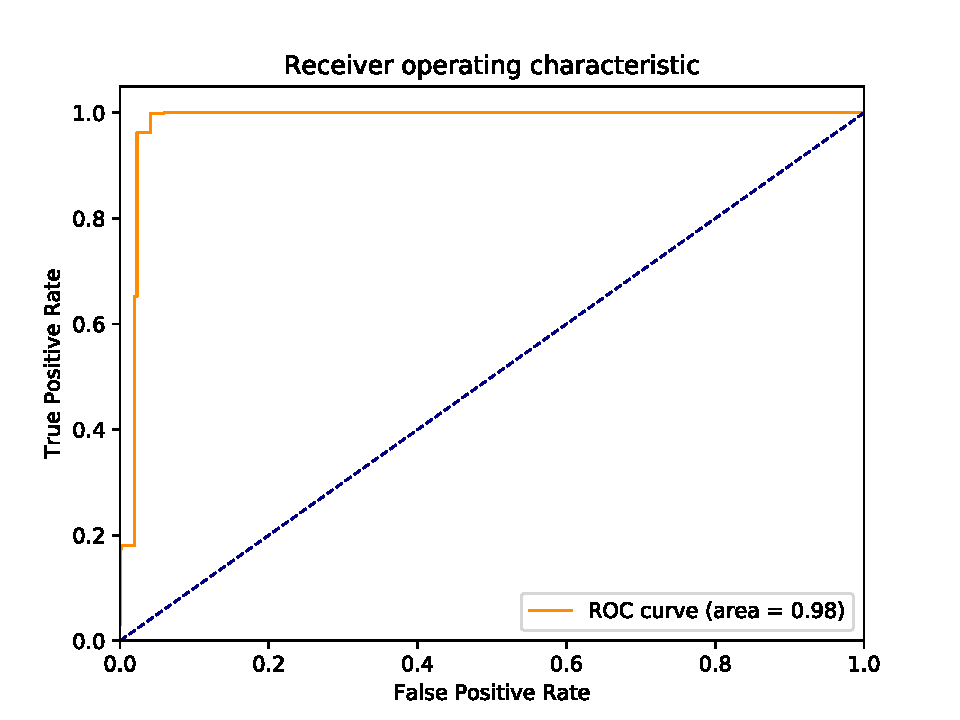
\includegraphics[scale=0.25]{roc-curve-full-dataset-ujratanitva.pdf}
			
			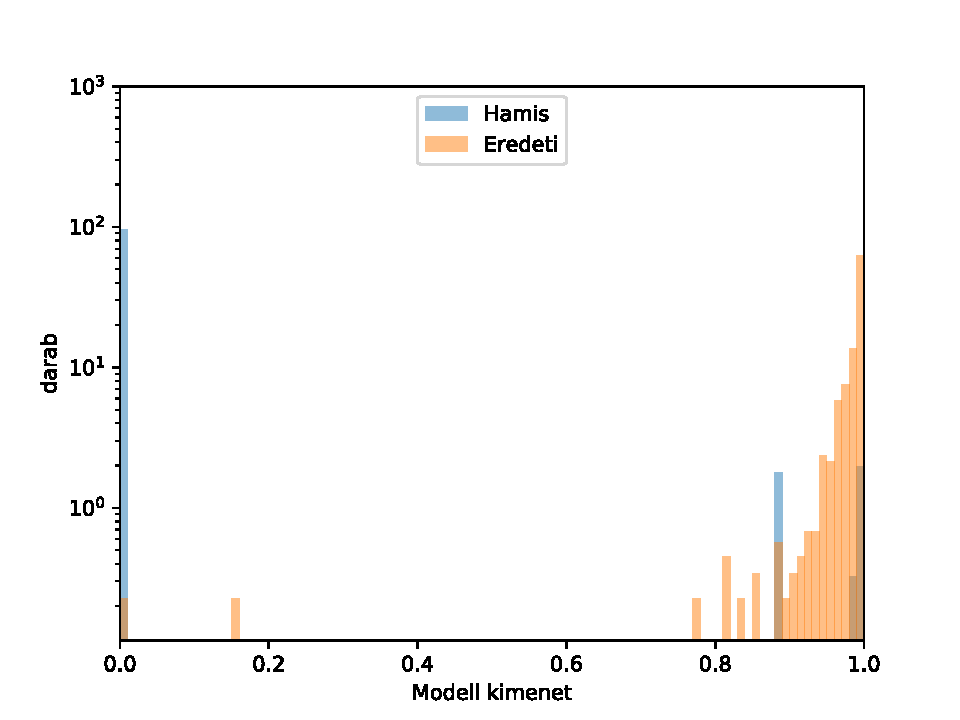
\includegraphics[scale=0.25]{histogram-ujratanitott-log-skala-full.pdf}
			
		\end{column}				
	\end{columns}



%	
%	\begin{figure}[ht]
%		
%		
%		\begin{minipage}[c]{0.3\linewidth}
%			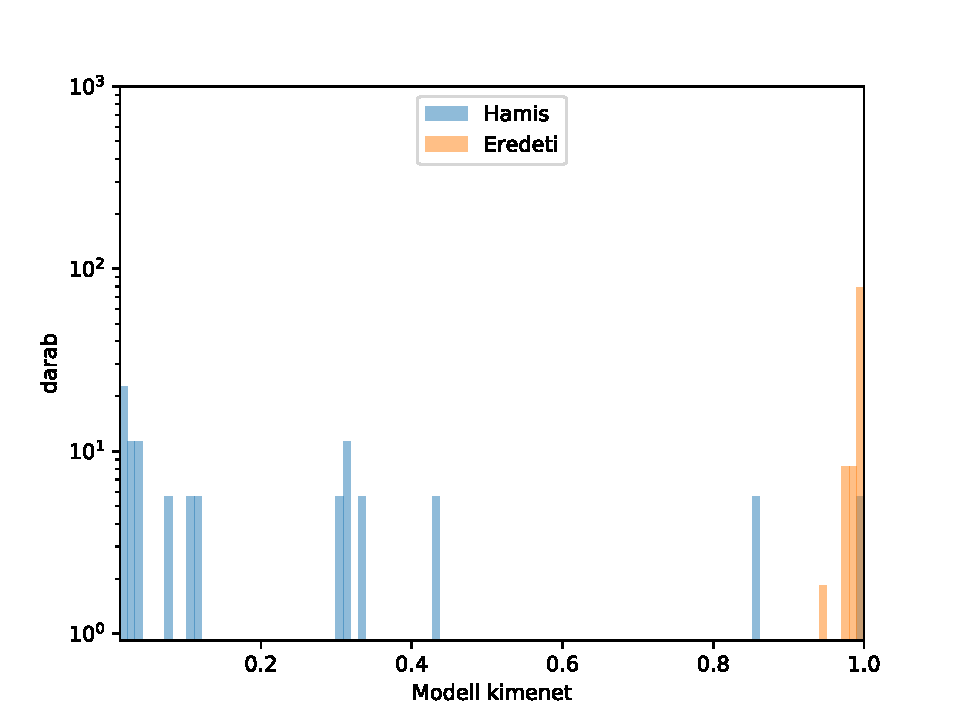
\includegraphics[scale=0.3]{histogram-ujratanitott-log-skala-test.pdf}
%			%		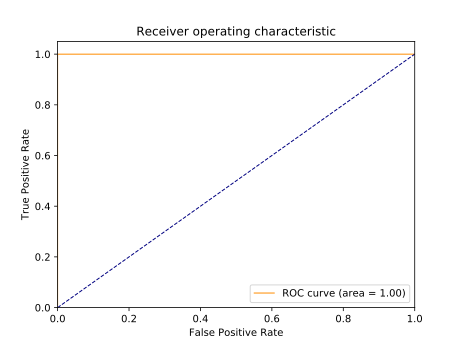
\includegraphics[width=\linewidth]{img/ruc-curve-test.svg}
%			\caption{Teszt halmaz.}
%			\label{fig:hist-test}
%			
%		\end{minipage}\hfill
%		\begin{minipage}[c]{0.3\linewidth}
%			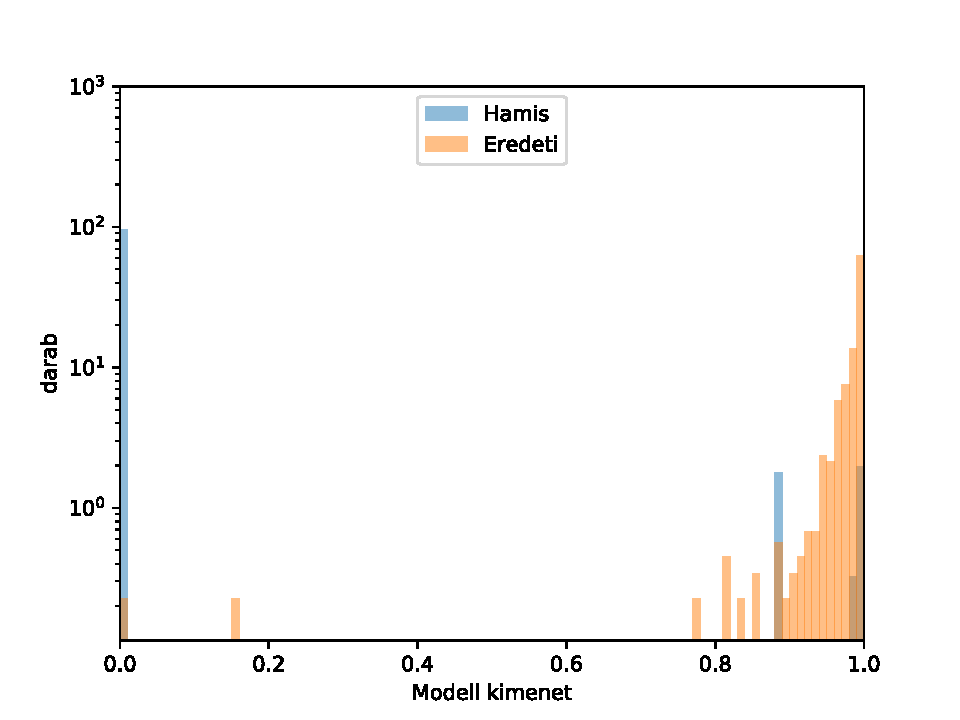
\includegraphics[scale=0.3]{histogram-ujratanitott-log-skala-full.pdf}
%			%		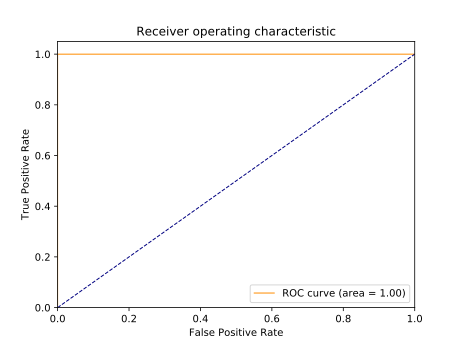
\includegraphics[width=\linewidth]{img/ruc-curve-test.svg}
%			\caption{Tanító+Teszt adathalmaz.}\label{fig:hist-full}
%			
%		\end{minipage}
%		%	\caption{\textbf{Az újratanított háló predikciós hisztogramja}}
%		\label{fig:histogram-ujratanitott}
%	\end{figure}


\end{frame}


\begin{frame}
	\frametitle{Mély konvolúciós hálók}
	\framesubtitle{Eredmények}

	A mély konvolúciós háló eredményei:
	
	\begin{figure} [h!]
		\centering
		\begin{tabular}{ l c c c c  }
			\underline{Módszer} 			& Összes(db) 	& Bizonytalan	& FP	& FN \\
			\texttt{bpas-verdict.csv} 	& 959 			& 0.21			& 0.10215 	& 0.00905 	\\
			\texttt{bpas-merged.csv}  	& 496			& 0.10			& 0.14545 	& 0.00259   \\
			
			\hline
			Konv. háló redukálva\footnotemark 	& 894			& 0				& 0.02798	& 0.00972	\\
			Konv. háló újratanítva& 894			& 0				& 0.05555	& 0.00900	\\
			
			
		\end{tabular} 
		
%		\caption{A mély konvolúciós háló eredményei.}
		%	\caption{A mély konvolúciós háló eredményei összehasonlítva az eredeti algoritmusokéval}
	\end{figure}

%\addtocounter{footnote}{-1}
%\footnotetext{Lásd a \ref{sec:adatok} pontot.}
%\addtocounter{footnote}{1}
\footnotetext{A fentiek szerint szűrt mintákon.}
\end{frame}





\begin{frame}
	\frametitle{Konklúzió}
%	\framesubtitle{Eredmények}

	\begin{enumerate}
	\item SVM
		\begin{itemize}
			\item 
			Jobban működik, mint a kézzel írt algoritmus
			\item 
			Relatív kevés mintán is tud hatékonyan tanulni
			\item 
			Gyorsan tanítható
			\item
			Hasonló projektre könnyen újra felhasználható
		\end{itemize}
	
	\item
		Mély konvolúciós háló
		\begin{itemize}
		\item 
			A mély hálók ígéretesek de még vannak feladatok, valamint több mintaadat kell, hogy való életben is használható legyen
		\item 
			Lassan tanul
		\item
			Nem tudjuk belevinni a nyomdászi szakértelmet, mindent elölről tanul
		\end{itemize}
	\end{enumerate}


%	\begin{itemize}
%	\item 
%		Az SVM jobban működik, mint a kézzel írt algoritmus
%	\item 
%		A mély hálók ígéretesek de még vannak feladatok, valamint több mintaadat kell, hogy való életben is használható legyen
%	\end{itemize}
%	
%	majdm indjárt kitalálom ide mi jön
%	
%	-több minta
%	


\end{frame}



\begin{frame}

	\centering
	Köszönöm a figyelmet!

\end{frame}





\end{document}